%-----------------------------------------------------------------------------%
\chapter{\topikDua}
%-----------------------------------------------------------------------------%

%-----------------------------------------------------------------------------%
\section{Eksperimen}
%-----------------------------------------------------------------------------%
Pada bagian ini kami melakukan eksperimen perkalian matriks-vektor dan matriks bujursangkar pada CPU (sekuensial), CUDA, CUDA dengan \textit{shared memory}, CUBLAS dan CPU (\textit{cluster} MPI) untuk membandingkan kinerjanya.

\subsection{Perbandingan Program Sekuensial dan CUDA} 

Pada percobaan ini kami membuat membandingkan waktu eksekusi program perkalian matriks-vektor dan perkalian matriks bujursangkar sekuensial (CPU) dengan paralel CUDA (GPU). 

\subsubsection{Deskripsi Program}

\begin{enumerate}
	\item Program perkalian mariks-vektor/matriks bujursangkar sekuensial pada CPU \verb|mmul.c|\footnote{\url{https://github.com/yohanesgultom/parallel-programming-assignment/blob/master/PR3/problem2/mmul.c}} dengan cara penggunaan program:
	
	\begin{lstlisting}
	$ mmul.c [baris/kolom matrix] [baris vektor] 1 [repetisi]
	\end{lstlisting}
	
	Argumen program:
	\begin{enumerate}
		\item Baris/kolom matriks: ukuran baris atau kolom matriks bujursangkar
		\item Baris vektor: ukuran vektor
		\item Repetisi: banyaknya perkalian diulang (untuk diambil rata-ratanya)
	\end{enumerate}
	
	\begin{lstlisting}
	$ mmul.c [baris matrix A] [kolom matriks A/baris matriks B] [kolom matriks B] [repetisi]
	\end{lstlisting}
	
	Argumen program:
	\begin{enumerate}
		\item Baris matriks A: ukuran baris atau kolom matriks bujursangkar
		\item Kolom matriks A/baris matriks B: ukuran kolom matriks A/baris matriks B
		\item Repetisi: banyaknya perkalian diulang (untuk diambil rata-ratanya)
	\end{enumerate}
	
	\item Program perkalian mariks-vektor/matriks bujursangkar paralel dengan CUDA \verb|mmul_cuda.cu|\footnote{\url{https://github.com/yohanesgultom/parallel-programming-assignment/blob/master/PR3/problem2/mmul_cuda.cu}}. Program ini diadaptasi dari satu sumber eksternal\footnote{\url{Sumber: https://gist.github.com/wh5a/4313739}}. Cara penggunaannya:
	
	\begin{lstlisting}
	$ mmul_cuda.cu [baris/kolom matrix] [baris vektor] 1 0 [repetisi]
	\end{lstlisting}
	
	Argumen program:
	\begin{enumerate}
		\item Baris/kolom matriks: ukuran baris atau kolom matriks bujursangkar
		\item Baris vektor: ukuran vektor
		\item Repetisi: banyaknya perkalian diulang (untuk diambil rata-ratanya)
	\end{enumerate}

	\begin{lstlisting}
	$ mmul_cuda.cu [baris matrix A] [kolom matriks A/baris matriks B] [kolom matriks B] [repetisi]
	\end{lstlisting}
	
	Argumen program:
	\begin{enumerate}
		\item Baris matriks A: ukuran baris atau kolom matriks bujursangkar
		\item Kolom matriks A/baris matriks B: ukuran kolom matriks A/baris matriks B
		\item Repetisi: banyaknya perkalian diulang (untuk diambil rata-ratanya)
	\end{enumerate}
	
	Program \verb|mmul_cuda.cu| ini memiliki ukuran \textit{threads/block} tetap yaitu \verb|(TILE_WIDTH, TILE_WIDTH)| dengan nilai \verb|TILE_WIDTH = 10|. Sedangkan ukuran \textit{grid} akan bergantung pada ukuran matriks/vektor dengan rumus:
	
	\begin{lstlisting}
	GRID SIZE = ((baris vektor-1) / TILE_WIDTH + 1, (baris matriks-1) / TILE_WIDTH + 1)
	\end{lstlisting}
	
\end{enumerate}

\subsubsection{Hasil Eksperimen}

Hasil eksekusi program perkalian matriks-vektor sekuensial dan CUDA (pada GPU 940M) dapat dilihat pada grafik gambar \ref{fig:seq_cuda_mv_940}. Pada gambar tersebut terlihat bahwa waktu eksekusi program sekuensial dan CUDA masih sama dengan ukuran data 10.000 (matriks $10.000 \times 10.000$ dan vektor $10.000$) hingga 15.000. Tapi pada ukuran data 20.000 hingga 40.000 terlihat bahwa program CUDA membutuhkan waktu yang lebih sedikit dibanding program sekuensial. Pada ukuran data terbesar di eksperimen ini, terlihat bahwa waktu yang dibutuhkan CUDA hanyalah $\nicefrac{1}{2}$ dari program sekuensial.

\begin{figure}
	\centering
	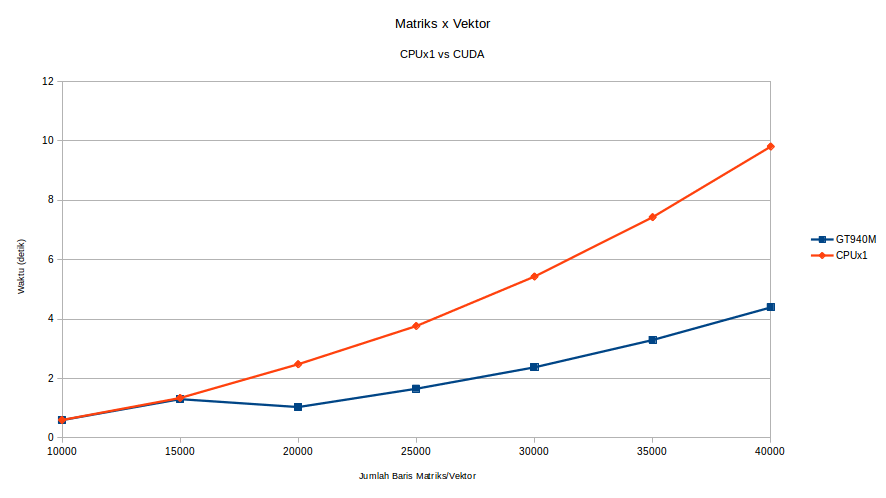
\includegraphics[width=1\textwidth]
	{pics/seq_cuda_mv_940}
	\caption{Waktu eksekusi program matriks x vektor sekuensial dan CUDA}
	\label{fig:seq_cuda_mv_940}
\end{figure}  

Perbedaan waktu eksekusi terlihat semakin jelas pada hasil eksekusi program perkalian matriks bujursangkar pada grafik gambar \ref{fig:seq_cuda_mm_940}. Waktu eksekusi program sekuensial dan CUDA hanya sama pada ukuran data 1.000 (perkalian dua matriks $1.000 \times 1.000$). Sedangkan untuk ukuran data 2.000 sampai 6.000, program CUDA membutuhkan waktu yang jauh lebih sedikit. Bahkan pada ukuran data terbesar di eksperimen ini, terlihat bahwa waktu yang dibutuhkan CUDA hanyalah $\nicefrac{1}{1000}$ dari program sekuensial.

\begin{figure}
	\centering
	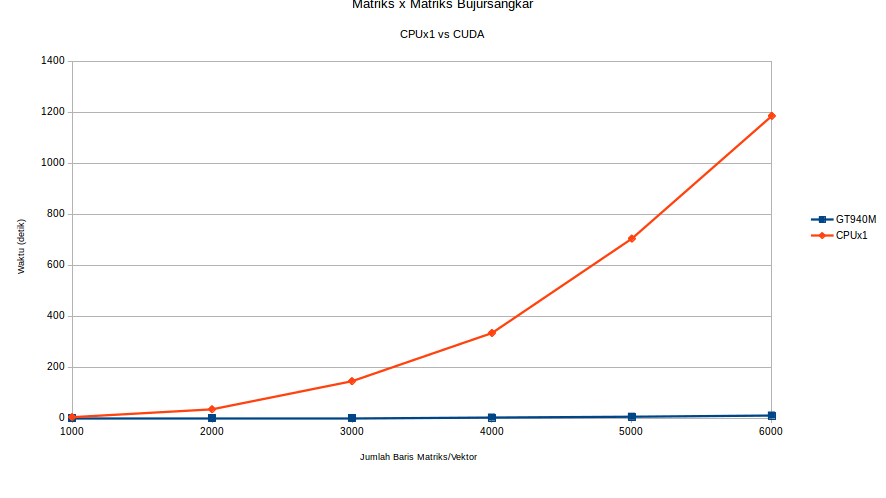
\includegraphics[width=1\textwidth]
	{pics/seq_cuda_mm_940}
	\caption{Waktu eksekusi program matriks x matriks sekuensial dan CUDA}
	\label{fig:seq_cuda_mm_940}
\end{figure}  

\subsection{Program CUDA dengan Variasi ukuran \textit{Grid}/\textit{Block}} 

Tujuan dari eksperimen ini adalah membandingkan kinerja perkalian matriks-vektor/matriks bujursangkar CUDA dengan variasi ukuran \textit{grid} dan \textit{block}.

\subsubsection{Deskripsi Program}

Ada tujuh buah program\footnote{\url{https://github.com/yohanesgultom/parallel-programming-assignment/tree/master/PR3/problem2}} yang digunakan pada eksperimen ini. Semua program ini diadaptasi dari satu sumber eksternal\footnote{\url{Sumber: https://gist.github.com/wh5a/4313739}}. Ketujuh program ini hanya dibedakan oleh nilai \verb|TILE_SIZE|-nya, yaitu sesuai dengan angka terakhir pada nama programnya (kecuali program \verb|mmul_cuda.cu| yang memiliki \verb|TILE_SIZE = 10|):
\begin{lstlisting}
$ mul_cuda.cu [baris A] [kolom A/baris B] [kolom B] 0 [repetisi]
$ mul_cuda_20.cu [baris A] [kolom A/baris B] [kolom B] 0 [repetisi]
$ mul_cuda_30.cu [baris A] [kolom A/baris B] [kolom B] 0 [repetisi]
$ mul_cuda_40.cu [baris A] [kolom A/baris B] [kolom B] 0 [repetisi]
$ mul_cuda_50.cu [baris A] [kolom A/baris B] [kolom B] 0 [repetisi]
$ mul_cuda_60.cu [baris A] [kolom A/baris B] [kolom B] 0 [repetisi]
$ mul_cuda_70.cu [baris A] [kolom A/baris B] [kolom B] 0 [repetisi]	
\end{lstlisting}

Seperti yang dijelaskan di eksperimen sebelumnya, program \verb|mmul_cuda.cu| dan \verb|mmul_cuda_XX.cu| ini memiliki ukuran \textit{threads/block} tetap yaitu \verb|(TILE_WIDTH, TILE_WIDTH)|. Sedangkan ukuran \textit{grid} akan bergantung pada ukuran matriks/vektor dengan rumus:

\begin{lstlisting}
GRID SIZE = ((baris vektor-1) / TILE_WIDTH + 1, (baris matriks-1) / TILE_WIDTH + 1)
\end{lstlisting}

\subsubsection{Hasil Eksperimen}

Eksperimen perkalian matriks-vektor CUDA dengan ukuran data tetap (matriks $5.000 \times 5.000$ dan vektor $5.000$) variasi ukuran \textit{block} dan \textit{grid} pada tiga buah GPU (GTX 980, GTX 970 dan 940M) memberikan hasil seperti pada grafik gambar \ref{fig:block_grid_mv}. Hasil eksperimen menunjukkan bahwa tidak ada perbedaan signifikan ketika dilakukan variasi ukuran \textit{block} dan \textit{grid}. Hal ini terjadi secara konsisten di semua GPU yang digunakan.

\begin{figure}
	\centering
	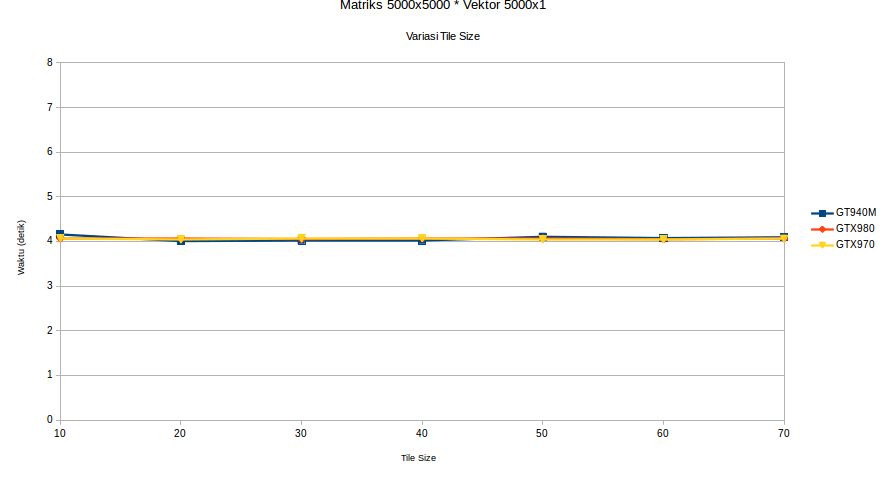
\includegraphics[width=1\textwidth]
	{pics/block_grid_mv}
	\caption{Waktu eksekusi program matriks x vektor CUDA dengan variasi ukuran \textit{block} dan \textit{grid}}
	\label{fig:block_grid_mv}
\end{figure}  

Sedangkan pada perkalian matriks bujursangkar (dua buah matriks $5.000 \times 5.000$) yang hasilnya ditunjukkan pada gambar \ref{fig:block_grid_mm}, terlihat adanya penurunan waktu eksekusi ketika ukuran \verb|TILE_SIZE| diperbesar (ukuran \textit{threads/block} semakin besar dan ukuran \textit{grid} semakin kecil). Tetapi ketika ukuran \verb|TILE_SIZE| dibuat lebih besar dari 40, tidak ada perubahan waktu eksekusi yang signifikan.

\begin{figure}
	\centering
	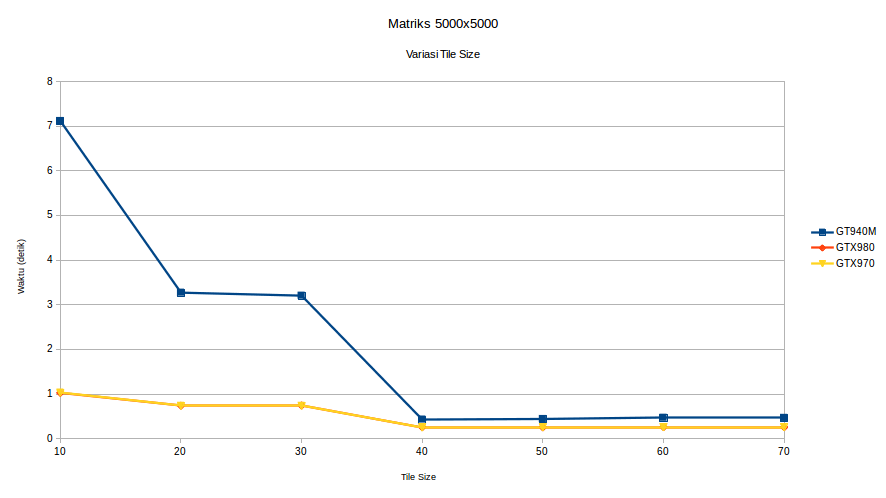
\includegraphics[width=1\textwidth]
	{pics/block_grid_mm}
	\caption{Waktu eksekusi program matriks bujursangkar CUDA dengan variasi ukuran \textit{block} dan \textit{grid}}
	\label{fig:block_grid_mm}
\end{figure}  

\subsection{Program CUDA \textit{Shared Memory}, CUBLAS dan MPI} 

Pada eksperimen ini akan diamati perbedaan waktu eksekusi program perkalian matriks-vektor CUDA yang hanya menggunakan \textit{global memory} (normal) dan yang menggunakan \textit{shared memory} (\textit{optimized}). Selain itu untuk kasus perkalian matriks bujursangkar, akan dibandingkan waktu eksekusi program CUDA dengan \textit{global memory} (normal), CUDA dengan \textit{shared memory} (\textit{optimized}), CUBLAS dan MPI (25 CPU pada \textit{cluster UCSD}).

\subsubsection{Deskripsi Program}

\begin{enumerate}

	\item Program perkalian mariks-vektor/matriks bujursangkar paralel dengan CUDA \verb|mmul_cuda.cu|\footnote{\url{https://github.com/yohanesgultom/parallel-programming-assignment/blob/master/PR3/problem2/mmul_cuda.cu}}. Program ini diadaptasi dari satu sumber eksternal\footnote{\url{Sumber: https://gist.github.com/wh5a/4313739}}. Cara penggunaannya:
	
	\begin{lstlisting}
	$ mmul_cuda.cu [baris A] [kolom A/baris B] [kolom B] 0 [repetisi] [optimized]​
	\end{lstlisting}
	
	Argumen program:
	\begin{enumerate}
		\item Baris matriks A: ukuran baris atau kolom matriks bujursangkar
		\item Kolom matriks A/baris matriks B: ukuran kolom matriks A/baris matriks B
		\item Repetisi: banyaknya perkalian diulang (untuk diambil rata-ratanya)
		\item \textit{Optimized}: menggunakan \textit{global memory} saja (0) atau optimasi dengan \textit{shared memory} (1)
	\end{enumerate}
	
	Program \verb|mmul_cuda.cu| ini memiliki ukuran \textit{threads/block} tetap yaitu \verb|(TILE_WIDTH, TILE_WIDTH)| dengan nilai \verb|TILE_WIDTH = 10|. Sedangkan ukuran \textit{grid} akan bergantung pada ukuran matriks/vektor dengan rumus:
	
	\begin{lstlisting}
	GRID SIZE = ((baris vektor-1) / TILE_WIDTH + 1, (baris matriks-1) / TILE_WIDTH + 1)
	\end{lstlisting}
	
	\item Program perkalian mariks-vektor/matriks bujursangkar paralel dengan CUBLAS \verb|mmul_cublas.cu|\footnote{\url{https://github.com/yohanesgultom/parallel-programming-assignment/blob/master/PR3/problem2/mmul_cublas.cu}}. Program ini diadaptasi dari satu sumber eksternal\footnote{\url{https://raw.githubusercontent.com/sol-prog/cuda_cublas_curand_thrust/master/mmul_1.cu}}. Cara penggunaannya:
	
	\begin{lstlisting}
	$ mmul_cublas.cu [baris A] [kolom A/baris B] [kolom B] [repetisi]
	\end{lstlisting}
	
	Argumen program:
	\begin{enumerate}
		\item Baris matriks A: ukuran baris atau kolom matriks bujursangkar
		\item Kolom matriks A/baris matriks B: ukuran kolom matriks A/baris matriks B
		\item Repetisi: banyaknya perkalian diulang (untuk diambil rata-ratanya)
	\end{enumerate}

	\item Program perkalian mariks-vektor/matriks bujursangkar paralel dengan MPI \verb|mmul_rowwise.c|\footnote{\url{https://github.com/yohanesgultom/parallel-programming-assignment/blob/master/PR3/problem2/mmul_rowwise.c}}. Cara penggunaannya:
	
	\begin{lstlisting}
	$ mmul_rowwise.c [baris A] [kolom A/baris B] [kolom B]
	\end{lstlisting}
	
	Argumen program:
	\begin{enumerate}
		\item Baris matriks A: ukuran baris atau kolom matriks bujursangkar
		\item Kolom matriks A/baris matriks B: ukuran kolom matriks A/baris matriks B
	\end{enumerate}
		
\end{enumerate}

\subsubsection{Hasil Eksperimen}

Seperti yang terlihat pada gambar \ref{fig:shared_cuda_mv_940}, hasil eksekusi perkalian matriks-vektor CUDA yang hanya menggunakan \textit{global memory} dan yang dioptimasi dengan menggunakan \textit{shared memory} pada GPU 940M menunjukkan bahwa optimasi dengan \textit{shared memory} hanya mengurangi waktu eksekusi untuk ukuran data di bawah 20.000 (matriks $20.000 \times 20.000$ dan vektor 20.000). Sedangkan untuk ukuran yang lebih besar waktu eksekusinya sama.

\begin{figure}
	\centering
	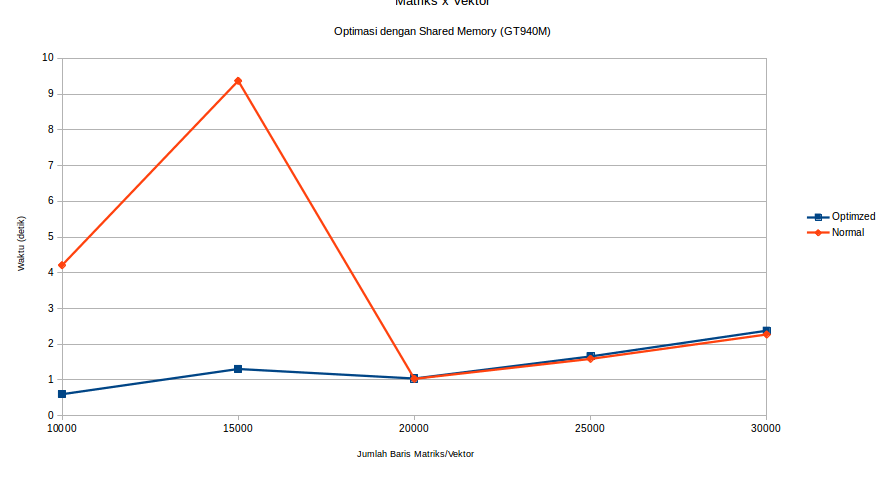
\includegraphics[width=1\textwidth]
	{pics/shared_cuda_mv_940}
	\caption{Waktu eksekusi program matriks x vektor \textit{global memory} dan \textit{shared memory} (940M)}
	\label{fig:shared_cuda_mv_940}
\end{figure}  

Hasil berbeda kami dapati pada GPU GTX 970 (gambar \ref{fig:shared_cuda_mv_970}) dan GTX 980 (gambar \ref{fig:shared_cuda_mv_980}) di mana program perkalian matriks-vektor dengan \textit{shared memory} selalu lebih cepat (0,5-3 detik) dari program yang hanya menggunakan \textit{global memory}. Menurut kami hal ini disebabkan karena sumber daya GPU 940M juga dipakai oleh OS mesinnya untuk menampilkan \textit{Graphical User Interface} (GUI). Di mana untuk GPU lainnya, OS yang digunakan tidak menggunakan GUI sehingga sumber daya GPU hanya digunakan oleh program CUDA.

\begin{figure}
	\centering
	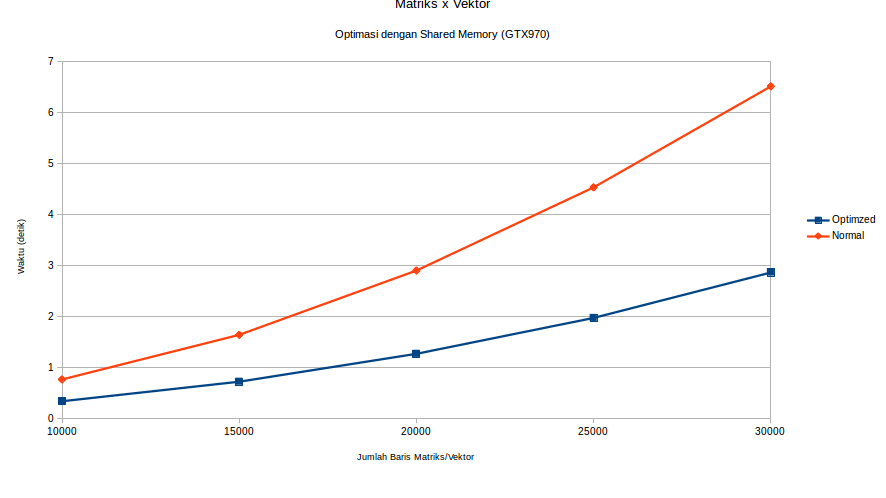
\includegraphics[width=1\textwidth]
	{pics/shared_cuda_mv_970}
	\caption{Waktu eksekusi program matriks x vektor \textit{global memory} dan \textit{shared memory} (GTX 970)}
	\label{fig:shared_cuda_mv_970}
\end{figure}  

\begin{figure}
	\centering
	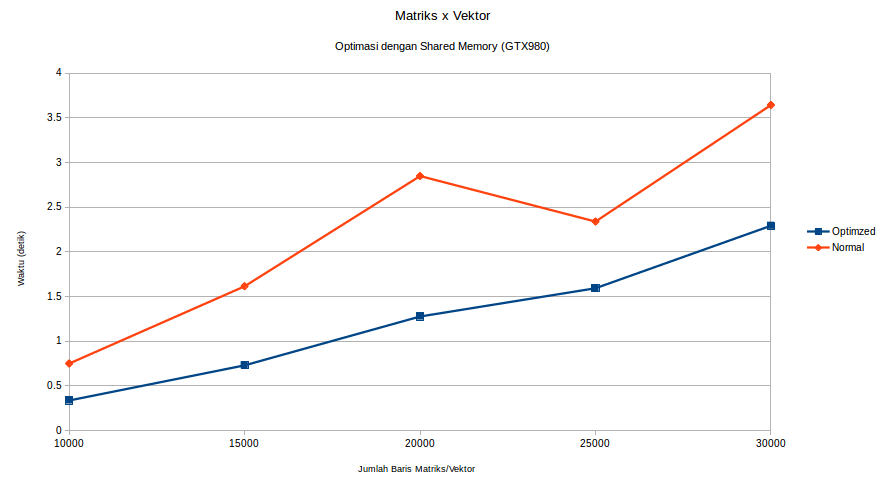
\includegraphics[width=1\textwidth]
	{pics/shared_cuda_mv_980}
	\caption{Waktu eksekusi program matriks x vektor \textit{global memory} dan \textit{shared memory} (GTX 980)}
	\label{fig:shared_cuda_mv_980}
\end{figure}  

Pada kasus perkalian matriks bujursangkar, perbandingan dilakukan sekaligus pada program CUDA dengan \textit{global memory}, CUDA dengan \textit{shared memory}, CUBLAS dan MPI. Pada GPU 940M (gambar \ref{fig:all_mm_940}) terlihat bahwa yang paling lambat adalah program CUDA dengan \textit{global memory} saja. Urutan program dari yang paling lambat sampai paling cepat adalah program CUDA dengan \textit{global memory} saja, MPI (\textit{cluster} 25 CPU), CUDA dengan \textit{shared memory} dan CUBLAS. Jika dilihat lebih rinci (gambar \ref{fig:all_shared_cublas_mm_940}), terlihat bahwa sebenarnya pada ukuran matriks di bawah 1.000, program CUDA dengan \textit{shared memory} sama cepat dengan CUBLAS. Baru pada ukuran lebih besar dari itu CUBLAS lebih cepat daripada program CUDA dengan \textit{shared memory}.

\begin{figure}
	\centering
	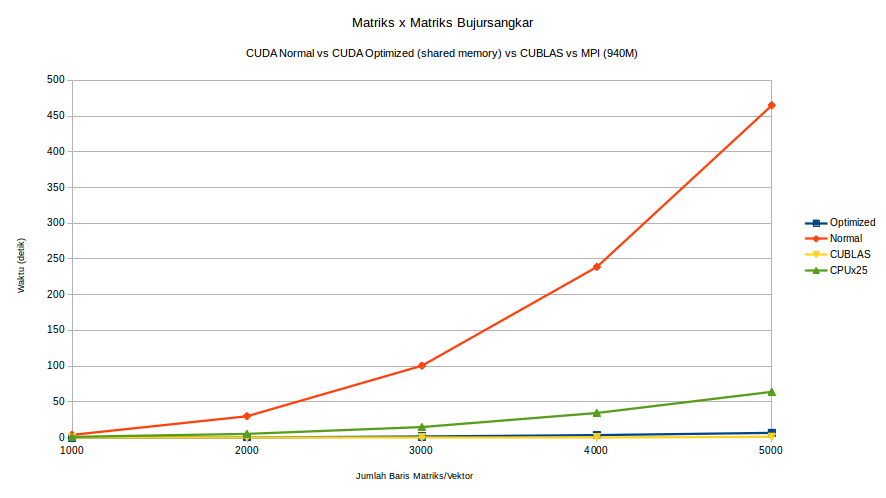
\includegraphics[width=1\textwidth]
	{pics/all_mm_940}
	\caption{Waktu eksekusi program perkalian matriks bujursangkar \textit{global memory}, \textit{shared memory}, CUBLAS dan MPI (940M)}
	\label{fig:all_mm_940}
\end{figure} 

\begin{figure}
	\centering
	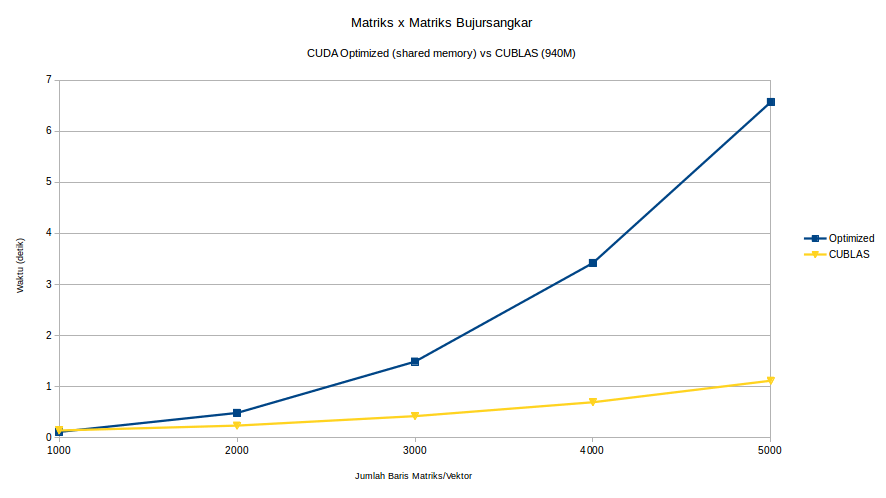
\includegraphics[width=1\textwidth]
	{pics/all_shared_cublas_mm_940}
	\caption{Waktu eksekusi program perkalian matriks bujursangkar \textit{shared memory} dan CUBLAS (940M)}
	\label{fig:all_shared_cublas_mm_940}
\end{figure} 

Hasil yang berbeda ditunjukkan pada perkalian matriks bujursangkar pada GTX 970 dan GTX 980 (gambar \ref{fig:all_mm_970} dan gambar \ref{fig:all_mm_980}), yaitu MPI (\textit{cluster} 25 CPU) adalah yang paling lambat dibanding yang lain. Setelah program MPI, urutan program yang terlambat hingga tercepat adalah CUDA dengan \textit{global memory}, CUDA dengan \textit{shared memory} dan CUBLAS. 

\begin{figure}
	\centering
	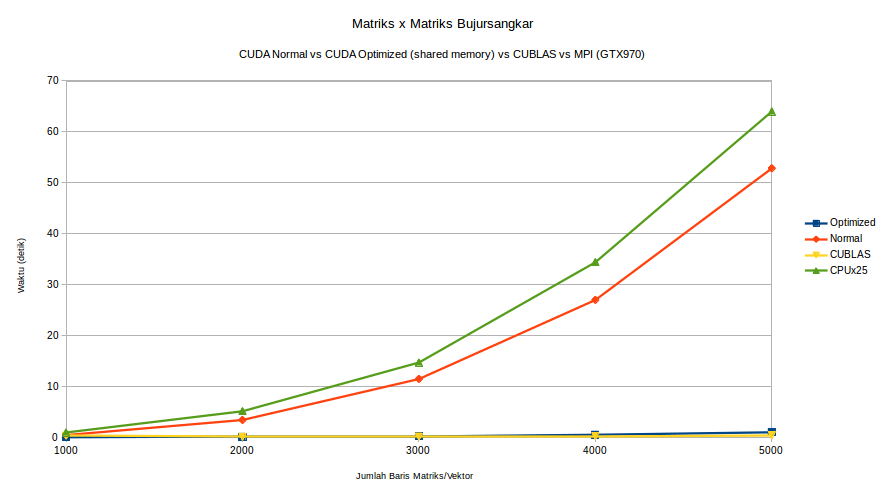
\includegraphics[width=1\textwidth]
	{pics/all_mm_970}
	\caption{Waktu eksekusi program perkalian matriks bujursangkar \textit{global memory}, \textit{shared memory}, CUBLAS dan MPI (GTX 970)}
	\label{fig:all_mm_970}
\end{figure} 

\begin{figure}
	\centering
	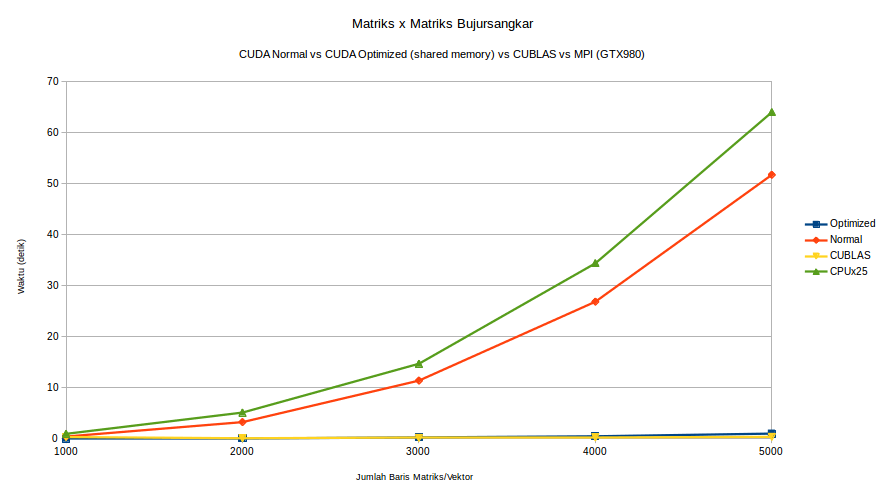
\includegraphics[width=1\textwidth]
	{pics/all_mm_980}
	\caption{Waktu eksekusi program perkalian matriks bujursangkar \textit{global memory}, \textit{shared memory}, CUBLAS dan MPI (GTX 980)}
	\label{fig:all_mm_980}
\end{figure} 

Hasil perbandingan waktu eksekusi perkalian matriks bujursangkar CUDA dengan \textit{shared memory} dan CUBLAS pada GTX 970 dan GTX 980 (gambar \ref{fig:all_shared_cublas_mm_970} dan gambar \ref{fig:all_mm_980}) ternyata agak mirip dengan hasil pada 940M (gambar \ref{fig:all_shared_cublas_mm_940}), yaitu CUBLAS lebih cepat dari CUDA dengan \textit{shared memory} pada ukuran matriks yang besar (dalam eksperimen ini lebih besar dari 2.000).

\begin{figure}
	\centering
	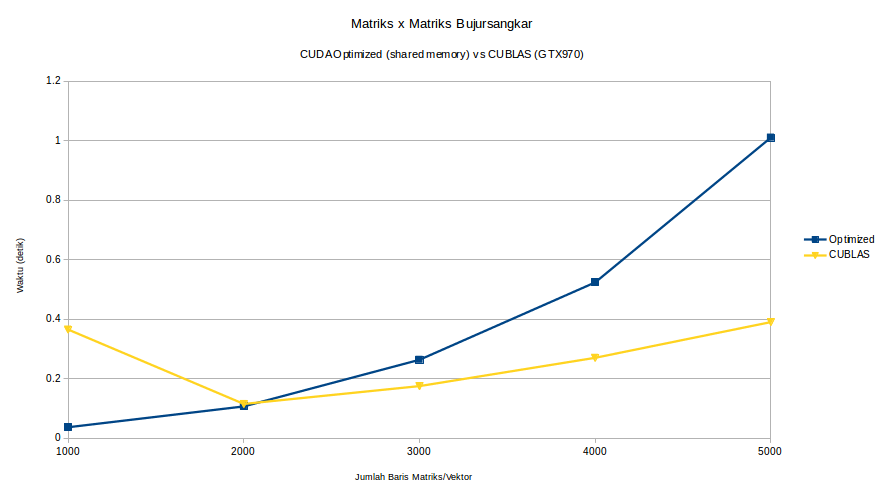
\includegraphics[width=1\textwidth]
	{pics/all_shared_cublas_mm_970}
	\caption{Waktu eksekusi program perkalian matriks bujursangkar \textit{shared memory} dan CUBLAS (970)}
	\label{fig:all_shared_cublas_mm_970}
\end{figure} 

\begin{figure}
	\centering
	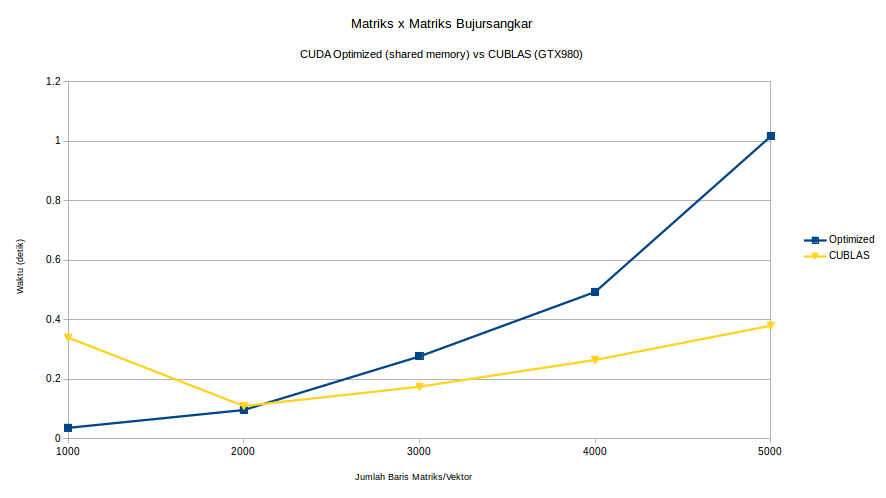
\includegraphics[width=1\textwidth]
	{pics/all_shared_cublas_mm_980}
	\caption{Waktu eksekusi program perkalian matriks bujursangkar \textit{shared memory} dan CUBLAS (980)}
	\label{fig:all_shared_cublas_mm_980}
\end{figure} 

%-----------------------------------------------------------------------------%
\section{Kesimpulan}
%-----------------------------------------------------------------------------%

Berdasarkan hasil eksperimen di atas, kami menarik beberapa kesimpulan:

\begin{enumerate}	
	\item GPU (CUDA) lebih cepat dari CPU (baik sekuensial maupun paralel dengan MPI) untuk kasus perkalian matriks/vektor dengan banyak elemen (dan operasi)
	\item Program CUDA dapat dioptimasi dengan menggunakan \textit{shared memory} karena \textit{shared memory} dapat diakses lebih cepat dari \textit{global memory}
	\item Dalam kasus dunia nyata, penggunaan library CUBLAS untuk melakukan operasi matriks/vektor lebih disarankan karena sudah dioptimasi khususnya untuk operasi terhadap data yang sangat besar
	\item Jika menggunakan CUDA perlu diperhatikan konfigurasi ukuran \textit{block} dan \textit{grid} yang optimal untuk algoritma dan arsitektur GPU yang dipakai karena pada operasi perkalian matriks bujursangkar waktu proses akan lebih lambat jika konfigurasi tidak sesuai
\end{enumerate}